\subsection{Definitions}

\begin{description}
	\item[Simulation] is the imitation of the operation of a real world process or system over time (e.g. via MATLAB/Simulink)
	\item[Hardware in the loop (HiL)] means testing of software in combination with an existing hardware component OR: HiL is a technique for testing a embedded system by simulating the real environment around the embedded system. \figref{fig:HiL}
		\begin{figure}[!h]
		\centering
			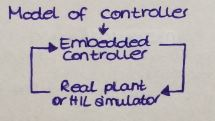
\includegraphics[width=0.4\linewidth]{HiL}
			\caption{Hardware in the loop (HiL)}
			\label{fig:HiL}
		\end{figure}
	\item[Software in the loop (SiL)] is a simulation technique for software models only with a simulated hardware and not with a realworld existing hardware OR SiL is a technique for testing software by simulating the target hardware \figref{fig:SiL}.
		\begin{figure}[!h]
			\centering
			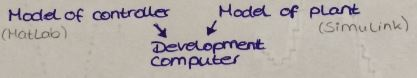
\includegraphics[width=0.7\linewidth]{SiL}
			\caption{Software in the loop (SiL)}
			\label{fig:SiL}
		\end{figure}
	\item[Model] is an abstraction from realworld objects; mostly easier to display.
	\item[Fourier-Transform] transforms time domain based signals into frequendy domain based signals; needed for calculation of signals
	\item[Time discrete] means that a signal is only defined at specifiv time values \figref{fig:timediscrete}.
		\begin{figure}[!h]
			\centering
			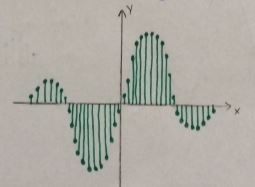
\includegraphics[width=0.5\linewidth]{timediscrete}
			\caption[Time discrete signal]{Time discrete signal: A y-value exists only for specific x-values.}
			\label{fig:timediscrete}
		\end{figure}
	\item[Time continuos] means that a signal is defined for the whole time or for an specific interval \figref{fig:timecontinuos}.
		\begin{figure}[!h]
			\centering
			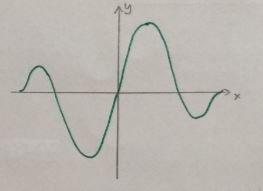
\includegraphics[width=0.7\linewidth]{timecontinuos}
			\caption[Time continuos signal]{Time continuos signal: A y-value exists for every x-value (in the intervall).}
			\label{fig:timecontinuos}
		\end{figure}
	\item[Discrete values] A signal can be measured in time ranges (time continuos) \figref{fig:discreteY_continuosX} or at specific time values (time discrete)\figref{fig:discreteY_discreteX}. Each y-value in one time range has got the same value. Discrete values can be counted.
		\begin{figure}[!h]
			\centering
			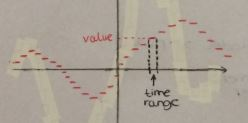
\includegraphics[width=0.7\linewidth]{discreteY_continuosX}
			\caption[Continuos X, discrete Y]{Continuos X, discrete Y}
			\label{fig:discreteY_continuosX}
		\end{figure}
		
		\begin{figure}[!h]
			\centering
			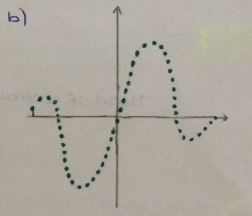
\includegraphics[width=0.7\linewidth]{discreteY_discreteX}
			\caption[Discrete X, discrete Y]{Discrete X, discrete Y}
			\label{fig:discreteY_discreteX}
		\end{figure}

	\item[Continuos values] can be measured and can take any value (\figref{fig:ContinuosX_continuosY} and \figref{fig:DiscreteX_continuosY})
		\begin{figure}[!h]
			\centering
			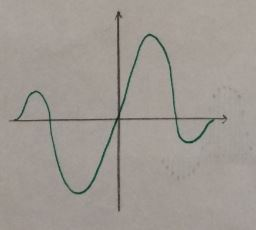
\includegraphics[width=0.7\linewidth]{ContinuosX_continuosY}
			\caption{Continuos X, discrete Y}
			\label{fig:ContinuosX_continuosY}
		\end{figure}
		
		\begin{figure}[!h]
			\centering
			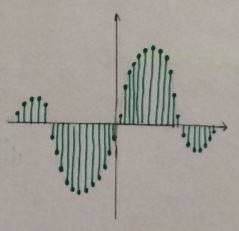
\includegraphics[width=0.7\linewidth]{DiscreteX_continuosY}
			\caption{Discrete X, continuos Y}
			\label{fig:DiscreteX_continuosY}
		\end{figure}
		
	\item[Discrete Fourier Transform (DFT)] is a stand alone definition for time discrete signals of limited duration besides the Fourier Transform \figref{fig:DFT}.
		\begin{figure}[!h]
			\centering
			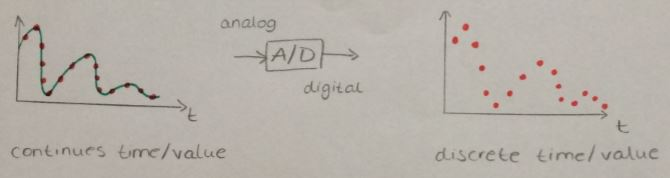
\includegraphics[width=0.7\linewidth]{DFT}
			\caption[Discrete Fourier Transform (DFT)]{Discrete Fourier Transform (DFT)}
			\label{fig:DFT}
		\end{figure}
	\item[Dirac distribution] $\dirac$ ist not function, but a distribution. It cannot be defined directly, but has to be described indirectly e.g. by intregration.
		\begin{enumerate}
			\item $ \dirac=0$ for all $t\neq0$ and $\int_{-\infty}^{+\infty}\dirac dt = 1 $
				\begin{figure}[!h]
					\centering
					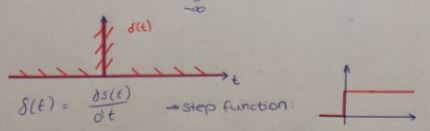
\includegraphics[width=0.7\linewidth]{dirac1}
					\caption{Dirac}
					\label{fig:dirac1}
				\end{figure}
			\item Sifting property (similar to window function)
			$\int_{-\infty}^{+\infty} f(t) \cdot \dirac dt = f(0) $
			\item $\dirac = \int_{-\infty}^{+\infty}(\lim\limits_{n \to \infty} \frac{1}{2\varepsilon}[s(t+\varepsilon)-s(t-\varepsilon)] ); \varepsilon>0 $
				\begin{figure}[!h]
					\centering
					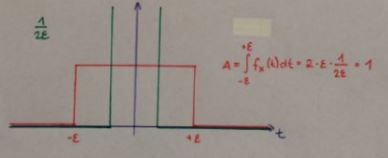
\includegraphics[width=0.7\linewidth]{dirac2}
					\caption{Dirac2}
					\label{fig:dirac2}
				\end{figure}				
		\end{enumerate}
	\item[Dirac comb ${III}_1$] is a periodic funtion of the Dirac distribution. The ideal sampling can be described by Dirac distributions located with distances $T_s$ which results in a spectrum of Dirac distributions having the distance $\frac{1}{T_s}$ \figref{fig:diraccomb}.
		\begin{figure}[!h]
			\centering
			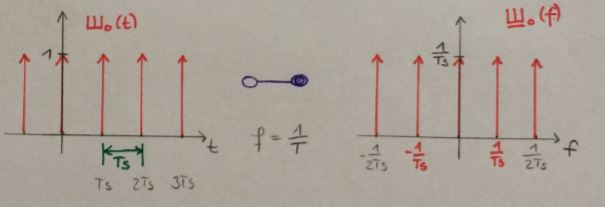
\includegraphics[width=0.7\linewidth]{diraccomb}
			\caption{Dirac Comb}
			\label{fig:diraccomb}
		\end{figure}
	\item[Algorithm] is a self-contained step by step set of operations to be performed in order to get a solution. Algorithms perform calculations, data processing and/or automated reasoning tasks.
	\item[DFT/FFT] The Fast Fourier Transform (FFT) is a special algorithm for calculating the DFT.
	\item[Sequence] is a ordered collection of objects in which repetitions are allowed. The number of elements is called the length $n$ of a sequence and can be infinite. The position of the elements is called index.
	E.g. prim numbers until 41: 
	
	\begin{tabular}{rccccccc} 
		prim numbers &2 & 3 & 5 & 7 & ... & 37 & 41 \\  
		& $\downarrow$ & $\downarrow$ & $\downarrow$ & $\downarrow$ &  & $\downarrow$ &   $\downarrow$ \\ 
		index & 1 & 2 & 3 & 4 & ...   & 12 & 13 \\ 
	\end{tabular} 
	
	The Length of this sequence is $n=13$.
	
	\item[Sampling] converts a continuos time signal into a discrete time signal. Sampling is done by a multiplication of the signal $u(t)$ with the dirac comb. A multiplication in the time domain results in a convolution in frequency domain. It is performed over a limieted time.
	\item[Time domain and frequency domain] The function values of a signal in time domain depend on time values. In the frequency domain the function values depend n frequency values.
	
	$f(t) \laplace F(f)$ with $f=\frac{1}{t}$
	
	\item[Periodic funtion] repeats itself after a period of time. Examples: $\sin(x),\cos(x)$
	\item[Limited function] is only defined for a specific time range. A limieted function in time domain contains an unlimited spectrum of frequencies in frequency domain. 
	\item[Convolution] is a mathematical operation on two functions, similar to cross-correlation (system theory). The slution is a third function being the first function modified by the second one. Multiplication in time domain $\rightarrow$ Convolution in frequency domain.
	\item[Frequency spectrum] is a composition of different frequencies.
	\item[Amplitude spectrum] is the absolut value of a frequency spectrum OR is a composition of different amplitudes.
	\item[Discontinuities] appear where a function is not continuous \figref{fig:discontinu}.
		\begin{figure}
			\centering
			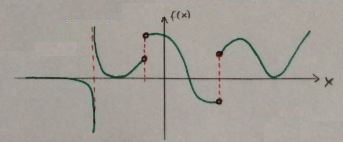
\includegraphics[width=0.7\linewidth]{discontinu}
			\caption{Example of a function with discontinuities}
			\label{fig:discontinu}
		\end{figure}
	

	\item[Sifting property of Dirac distribution] means that the function value $f(t=0)$ can be extracted with the mulitplication of the function with the Dirac distribution.
	
	$\int_{-\infty}^{+\infty} f(t) \cdot \dirac dt = f(0) $ 
	
	because of 
		
	$ \dirac=\left\{\begin{array}{ll} 0, & t \neq 0 \\
	\infty, & t = 0\end{array}\right. $	and $\int_{-\infty}^{+\infty}\dirac dt = 1 $
	
	\item[Window function] is a rectangular function used as a window for calculating a DFT. When a function is multiplied by a window function, the product is zero-valued outside of the window's interval; all that is left ist the part where they overlap, the "view though the window" \figref{fig:window}.
		\begin{figure}[!h]
			\centering
			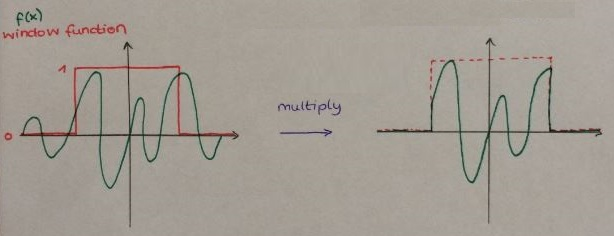
\includegraphics[width=0.7\linewidth]{window}
			\caption{Use of a window function}
			\label{fig:window}
		\end{figure}
	
	\item[Zero padding] adds zeros to the end of signals to compress the signal \figref{fig:zerop}.
		\begin{figure}[!h]
			\centering
			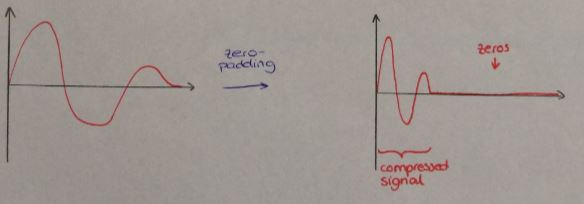
\includegraphics[width=0.7\linewidth]{zerop}
			\caption{Zero padding}
			\label{fig:zerop}
		\end{figure}


	
\end{description}
